% mnras_template.tex 
%
% LaTeX template for creating an MNRAS paper
%
% v3.0 released 14 May 2015
% (version numbers match those of mnras.cls)
%
% Copyright (C) Royal Astronomical Society 2015
% Authors:
% Keith T. Smith (Royal Astronomical Society)

% Change log
%
% v3.0 May 2015
%    Renamed to match the new package name
%    Version number matches mnras.cls
%    A few minor tweaks to wording
% v1.0 September 2013
%    Beta testing only - never publicly released
%    First version: a simple (ish) template for creating an MNRAS paper

%%%%%%%%%%%%%%%%%%%%%%%%%%%%%%%%%%%%%%%%%%%%%%%%%%
% Basic setup. Most papers should leave these options alone.
\documentclass[fleqn,usenatbib]{mnras} 

% MNRAS is set in Times font. If you don't have this installed (most LaTeX
% installations will be fine) or prefer the old Computer Modern fonts, comment
% out the following line
\usepackage{newtxtext,newtxmath}
% Depending on your LaTeX fonts installation, you might get better results with one of these:
%\usepackage{mathptmx}
%\usepackage{txfonts}

% Use vector fonts, so it zooms properly in on-screen viewing software
% Don't change these lines unless you know what you are doing
\usepackage[T1]{fontenc}

% Allow "Thomas van Noord" and "Simon de Laguarde" and alike to be sorted by "N" and "L" etc. in the bibliography.
% Write the name in the bibliography as "\VAN{Noord}{Van}{van} Noord, Thomas"
\DeclareRobustCommand{\VAN}[3]{#2}
\let\VANthebibliography\thebibliography
\def\thebibliography{\DeclareRobustCommand{\VAN}[3]{##3}\VANthebibliography}


%%%%% AUTHORS - PLACE YOUR OWN PACKAGES HERE %%%%%

% Only include extra packages if you really need them. Common packages are:
\usepackage{graphicx}	% Including figure files
\usepackage{amsmath}	% Advanced maths commands
\usepackage{amssymb}	% Extra maths symbols

%%%%%%%%%%%%%%%%%%%%%%%%%%%%%%%%%%%%%%%%%%%%%%%%%%

%%%%% AUTHORS - PLACE YOUR OWN COMMANDS HERE %%%%%

% Please keep new commands to a minimum, and use \newcommand not \def to avoid
% overwriting existing commands. Example:
%\newcommand{\pcm}{\,cm$^{-2}$}	% per cm-squared

\usepackage[dvipsnames]{xcolor}
\newcommand{\fk}[1]{{\bf \textcolor{PineGreen}{#1}}}		% Florians edit 

%%%%%%%%%%%%%%%%%%%%%%%%%%%%%%%%%%%%%%%%%%%%%%%%%%

%%%%%%%%%%%%%%%%%%% TITLE PAGE %%%%%%%%%%%%%%%%%%%

% Title of the paper, and the short title which is used in the headers.
% Keep the title short and informative.
\title[Supernova induced processing of interstellar dust]{Supernova induced processing of interstellar dust}

% The list of authors, and the short list which is used in the headers.
% If you need two or more lines of authors, add an extra line using \newauthor
\author[L. Mattsson et al.]{
L. Mattsson,$^{1}$\thanks{E-mail: lars.mattsson@su.se}
A. N. Other,$^{2}$
Third Author$^{2,3}$
and Fourth Author$^{3}$
\\
% List of institutions
$^{1}$Nordita, KTH Royal Institute of Technology and Stockholm University, Roslagstullsbacken 23, SE-106 91 Stockholm, Sweden\\
$^{2}$Department, Institution, Street Address, City Postal Code, Country\\
$^{3}$Another Department, Different Institution, Street Address, City Postal Code, Country
}

% These dates will be filled out by the publisher
\date{Accepted XXX. Received YYY; in original form ZZZ}

% Enter the current year, for the copyright statements etc.
\pubyear{2021}

% Don't change these lines
\begin{document}
\label{firstpage}
\pagerange{\pageref{firstpage}--\pageref{lastpage}}
\maketitle

% Abstract of the paper
\begin{abstract}
This is a simple template for authors to write new MNRAS papers.
The abstract should briefly describe the aims, methods, and main results of the paper.
It should be a single paragraph not more than 250 words (200 words for Letters).
No references should appear in the abstract.
\end{abstract}

% Select between one and six entries from the list of approved keywords.
% Don't make up new ones.
\begin{keywords}
keyword1 -- keyword2 -- keyword3
\end{keywords}

%%%%%%%%%%%%%%%%%%%%%%%%%%%%%%%%%%%%%%%%%%%%%%%%%%

%%%%%%%%%%%%%%%%% BODY OF PAPER %%%%%%%%%%%%%%%%%%

\section{Introduction}
\fk{Test.}

\newpage~
\newpage
\section{Hydrodynamic simulations}
 \begin{table}
 \centering
 \caption{List of hydrodynamics simulations}
 \begin{tabular}{ l l l}
 \hline\hline
 Index&Note&\\\hline 
 A&$n_\text{gas}=0.1\,\text{cm}^{-3}$, no turbulence&\\\hline  
 B&$n_\text{gas}=1.0\,\text{cm}^{-3}$, no turbulence&\\\hline   
 C&$n_\text{gas}=0.1\,\text{cm}^{-3}$, turbulence&\\\hline  
 D&$n_\text{gas}=1.0\,\text{cm}^{-3}$, turbulence&\\\hline   
 \end{tabular}
 \label{List_hydrosimulations}
 \end{table}

\newpage~
\newpage
 %######################################################################################################################  %######################################################################################################################
 %###################################################################################################################### 
\section{Dust processing}
 \begin{table}
 \centering
 \caption{List of dust post-processing simulations}
 \begin{tabular}{ l l l}
 \hline\hline
 Index&Note&\\\hline 
 1&Only transport&\\\hline  
 2&Transport + Sputtering + Grain-grain collisions&\\\hline 
 \end{tabular}
 \label{List_Dustsimulations}
 \end{table}
 
\newpage~
\newpage
 %######################################################################################################################  %######################################################################################################################
 %###################################################################################################################### 
\section{Results and discussion}

  \begin{figure*}
        \resizebox{\hsize}{!}{
      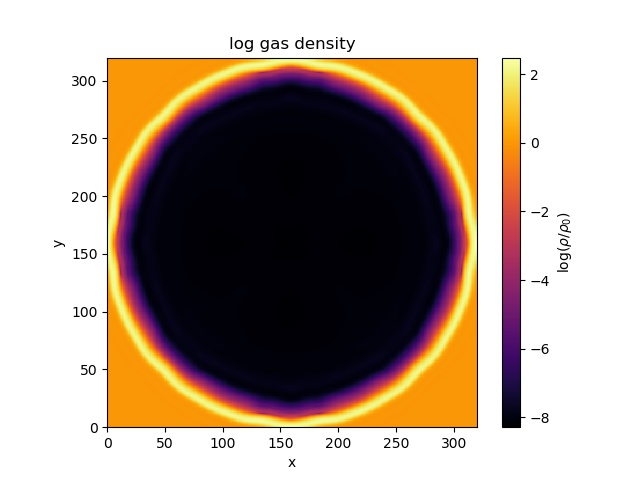
\includegraphics{3Dsedov_SN_dust_newsetup2_10pc_chi4_320_FGupd_rhoVAR60.jpg}
      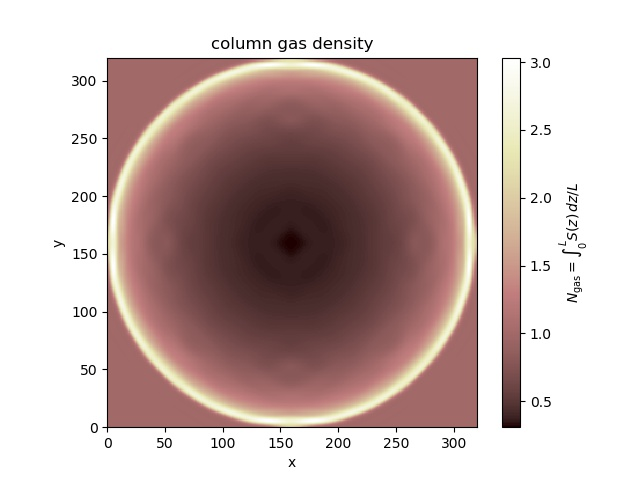
\includegraphics{3Dsedov_SN_dust_newsetup2_10pc_chi4_320_FGupd_column_gasVAR60.jpg}}
      \resizebox{\hsize}{!}{
      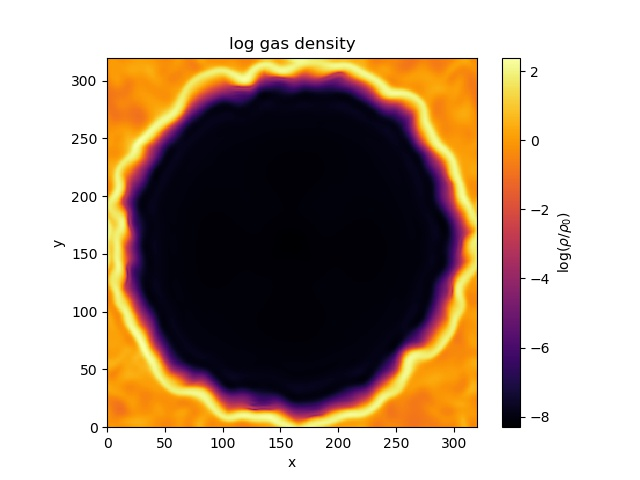
\includegraphics{3Dsedov_SN_dust_newsetup2_10pc_chi4_320_FGupd_uin2_rhoVAR60.jpg}
      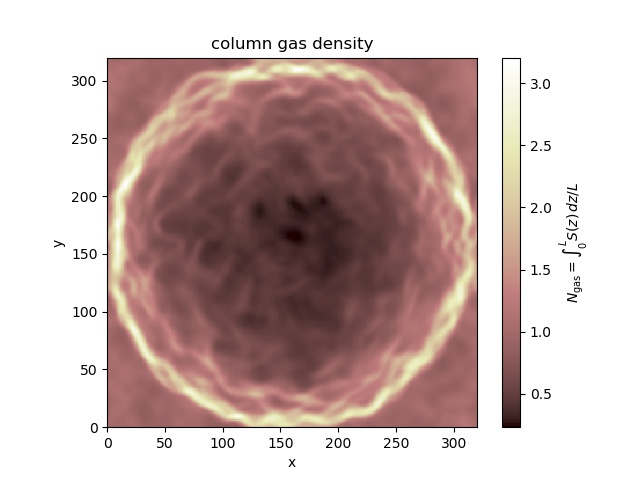
\includegraphics{3Dsedov_SN_dust_newsetup2_10pc_chi4_320_FGupd_uin2_column_gasVAR60.jpg}}

  \caption{\label{3Dsedov} }
  \end{figure*}  

  \begin{figure*}
        \resizebox{\hsize}{!}{
      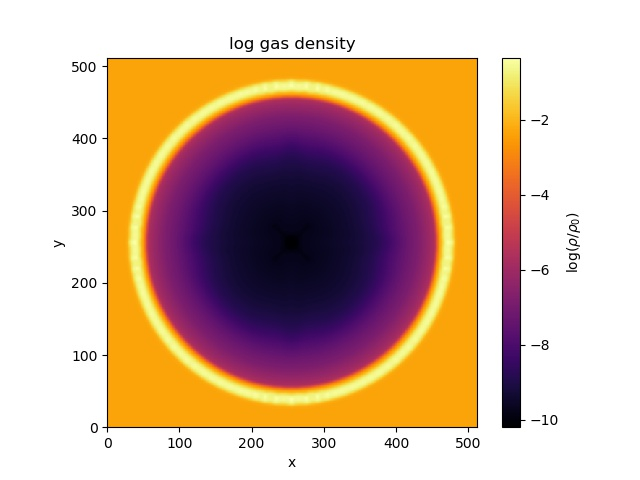
\includegraphics{3Dsedov_SN_dust_newsetup2_10pc_chi4_512_FGupd_new_n01_rhoVAR20.jpg}
      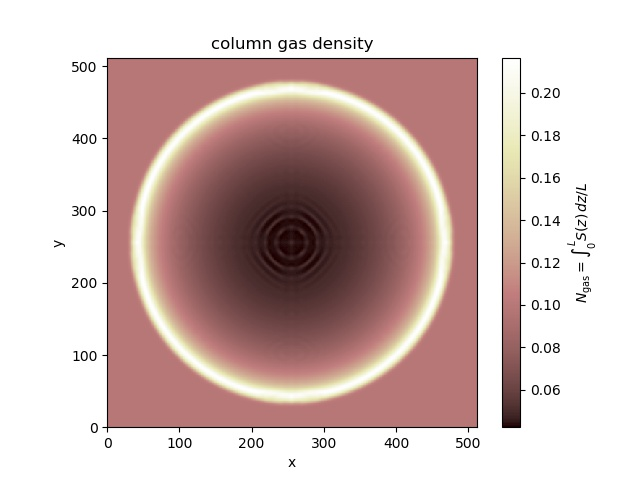
\includegraphics{3Dsedov_SN_dust_newsetup2_10pc_chi4_512_FGupd_new_n01_column_gasVAR20.jpg}}
      \resizebox{\hsize}{!}{
      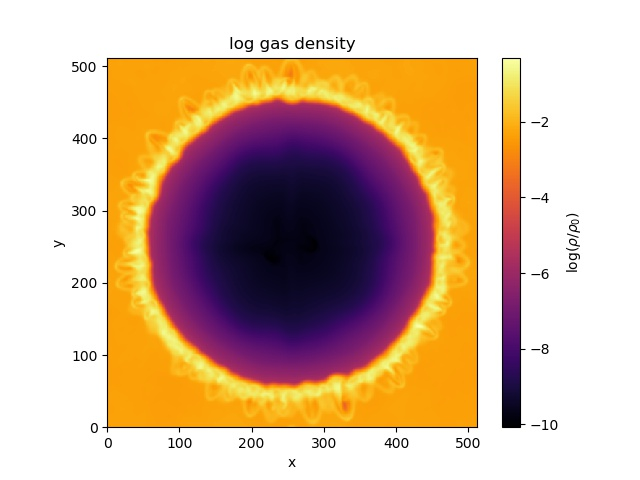
\includegraphics{3Dsedov_SN_dust_newsetup2_10pc_chi4_512_FGupd_new_n01_uin2_rhoVAR20.jpg}
      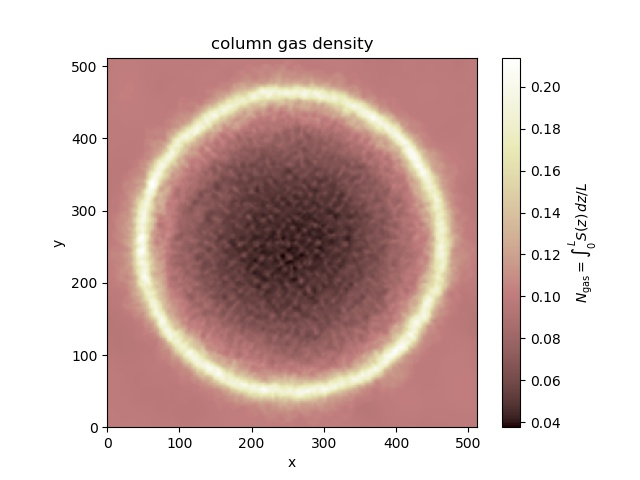
\includegraphics{3Dsedov_SN_dust_newsetup2_10pc_chi4_512_FGupd_new_n01_uin2_column_gasVAR20.jpg}}

  \caption{\label{3Dsedov} }
  \end{figure*}   

\section{Conclusions}


\section*{Acknowledgements}

The Acknowledgements section is not numbered. Here you can thank helpful
colleagues, acknowledge funding agencies, telescopes and facilities used etc.
Try to keep it short.

%%%%%%%%%%%%%%%%%%%%%%%%%%%%%%%%%%%%%%%%%%%%%%%%%%
\section*{Data Availability}

 
The inclusion of a Data Availability Statement is a requirement for articles published in MNRAS. Data Availability Statements provide a standardised format for readers to understand the availability of data underlying the research results described in the article. The statement may refer to original data generated in the course of the study or to third-party data analysed in the article. The statement should describe and provide means of access, where possible, by linking to the data or providing the required accession numbers for the relevant databases or DOIs.




%%%%%%%%%%%%%%%%%%%% REFERENCES %%%%%%%%%%%%%%%%%%

% The best way to enter references is to use BibTeX:

\bibliographystyle{mnras}
\bibliography{example} % if your bibtex file is called example.bib


% Alternatively you could enter them by hand, like this:
% This method is tedious and prone to error if you have lots of references
%\begin{thebibliography}{99}
%\bibitem[\protect\citeauthoryear{Author}{2012}]{Author2012}
%Author A.~N., 2013, Journal of Improbable Astronomy, 1, 1
%\bibitem[\protect\citeauthoryear{Others}{2013}]{Others2013}
%Others S., 2012, Journal of Interesting Stuff, 17, 198
%\end{thebibliography}

%%%%%%%%%%%%%%%%%%%%%%%%%%%%%%%%%%%%%%%%%%%%%%%%%%

%%%%%%%%%%%%%%%%% APPENDICES %%%%%%%%%%%%%%%%%%%%%

\appendix

\section{Some extra material}

If you want to present additional material which would interrupt the flow of the main paper,
it can be placed in an Appendix which appears after the list of references.

%%%%%%%%%%%%%%%%%%%%%%%%%%%%%%%%%%%%%%%%%%%%%%%%%%


% Don't change these lines
\bsp	% typesetting comment
\label{lastpage}
\end{document}

% End of mnras_template.tex
